% !Rnw root = main.Rnw


% !Rnw root = Introduction.Rnw
%===============================
\section{Using R}
%===============================
\begin{HIGHLIGHT}
\par\noindent{
R is an \emph{interactive} environment, wherein the users gets immediate feedback (\emph{results}) for their instructions (\emph{expressions}). This is in contrast to programming languages like C++ or Java wherein a set of instructions (the program) has to be created and compiled before the results can be generated.In R, the interaction between the user and the system constitutes an \emph{R Session}. During an R session, the user provides \emph{expressions} to R for doing computations, displaying results, and creating objects for further use. R, first evaluates the expressions for its syntactic correctness and then performs the task, as specified by the expression. We will examine some basic expressions in the following sub-sections.     
}
\end{HIGHLIGHT}

At the \emph{console}, the user finds the \textbf{$>$} prompt where the user responds by typing and expression. Hereon, in this section every expression/set of expressions is mentioned in the gray box and is to be issued at the $>$ prompt in the console. Moreover, following the motto of this course ``learn by doing``, the reader is strongly encouraged to try out each of these expressions and \emph{read the corresponding help manual for each expression}. As is evident from the examples shown in this section, expressions are predominantly \textbf{\emph{function calls with a set of arguments}}.

\begin{HIGHLIGHT}
\par\noindent{
R, like Python, MATLAB etc is a \emph{dynamically typed language} which means that you won't have to define the type of the variable (which stores your data). As a result, the user can only focus on the \emph{data stored by the variable} rather than having to worry about \emph{how the data is stored in the variable}. This is in stark contrast to \emph{statically typed languages} like C++ and Java.      
}
\end{HIGHLIGHT}

\begin{DIY}{Think}
How does a R \emph{data frame} exemplify the \emph{dynamic typing} feature of R?
\end{DIY}
    
\begin{DIY}{Warning}
The dynamic typing feature of R  provides great flexibility but at what cost?
\end{DIY}



% !Rnw root = Introduction.Rnw
\newpage
%===============================
\section{Basic Data Types}
%===============================
\begin{HIGHLIGHT}
\par\noindent{
Objects are the center of computations in R, along with the function calls that create and use those objects.
}
\end{HIGHLIGHT}

\begin{DIY}{Think}
What are objects in R? Why are functions and objects dual to each other? 
\end{DIY}

\subsubsection{The $class()$ function}
\noindent Every object in R has a \emph{type} associated with it, which signifies the kind of data it contains e.g numbers, strings etc. The $class()$ function accepts an object as an argument and returns its type.

\subsection{Data Type for Boolean}
\subsubsection{The ``logical'' type}
\begin{knitrout}
\definecolor{shadecolor}{rgb}{0.969, 0.969, 0.969}\color{fgcolor}\begin{kframe}
\begin{alltt}
\hlkwd{class}\hlstd{(}\hlnum{TRUE}\hlstd{)}
\end{alltt}
\begin{verbatim}
## [1] "logical"
\end{verbatim}
\begin{alltt}
\hlkwd{class}\hlstd{(}\hlnum{FALSE}\hlstd{)}
\end{alltt}
\begin{verbatim}
## [1] "logical"
\end{verbatim}
\end{kframe}
\end{knitrout}
\subsection{Data Type for Numbers}
\subsubsection{The ``numeric'' type}
\begin{knitrout}
\definecolor{shadecolor}{rgb}{0.969, 0.969, 0.969}\color{fgcolor}\begin{kframe}
\begin{alltt}
\hlkwd{class}\hlstd{(}\hlnum{1}\hlstd{)}
\end{alltt}
\begin{verbatim}
## [1] "numeric"
\end{verbatim}
\begin{alltt}
\hlkwd{class}\hlstd{(}\hlnum{3.141593}\hlstd{)}
\end{alltt}
\begin{verbatim}
## [1] "numeric"
\end{verbatim}
\end{kframe}
\end{knitrout}
\subsection{Data Type for Strings}
\subsubsection{The ``character'' type}
\begin{knitrout}
\definecolor{shadecolor}{rgb}{0.969, 0.969, 0.969}\color{fgcolor}\begin{kframe}
\begin{alltt}
\hlkwd{class}\hlstd{(}\hlstr{"Carpe Diem"}\hlstd{)}
\end{alltt}
\begin{verbatim}
## [1] "character"
\end{verbatim}
\end{kframe}
\end{knitrout}
\subsection{Concatenating Strings}
\subsubsection{The $paste()$ function}
\begin{knitrout}
\definecolor{shadecolor}{rgb}{0.969, 0.969, 0.969}\color{fgcolor}\begin{kframe}
\begin{alltt}
\hlkwd{paste}\hlstd{(}\hlstr{"Data Analysis"}\hlstd{,}\hlstr{"with R"}\hlstd{,}\hlkwc{sep}\hlstd{=}\hlstr{","}\hlstd{)}
\end{alltt}
\begin{verbatim}
## [1] "Data Analysis,with R"
\end{verbatim}
\end{kframe}
\end{knitrout}



% !Rnw root = Introduction.Rnw
%===============================
\section{Coercion}
%===============================
\begin{HIGHLIGHT}
\par\noindent{
{\centering\textbf{\emph{logical, integer, numeric, character}} \\}
\vspace{\baselineskip}
\noindent An ordering of data types from simple to complex. \emph{Coercion} is the conversion from one type to another. However, coercion from any type to another is neither possible nor valid. The general rule for coercion is: \emph{Coercion from a a simple type to a more complex type is valid}
}
\end{HIGHLIGHT}
\subsubsection{The ``is'' and ``as'' methods}
The \emph{is} method can be used to test whether an object is from a given class.

\noindent The \emph{as} method can be used to coerce an object from one class to another.
\subsection{Coercion between Boolean and Numbers}
\begin{knitrout}
\definecolor{shadecolor}{rgb}{0.969, 0.969, 0.969}\color{fgcolor}\begin{kframe}
\begin{alltt}
\hlkwd{is.logical}\hlstd{(}\hlnum{TRUE}\hlstd{)} \hlcom{##check if the  data is of type logical}
\end{alltt}
\begin{verbatim}
## [1] TRUE
\end{verbatim}
\begin{alltt}
\hlkwd{as.numeric}\hlstd{(}\hlnum{TRUE}\hlstd{)} \hlcom{##coerce from logical to numeric}
\end{alltt}
\begin{verbatim}
## [1] 1
\end{verbatim}
\begin{alltt}
\hlkwd{is.numeric}\hlstd{(}\hlnum{10}\hlstd{)} \hlcom{##check if the data is of type numeric}
\end{alltt}
\begin{verbatim}
## [1] TRUE
\end{verbatim}
\begin{alltt}
\hlkwd{as.logical}\hlstd{(}\hlnum{10}\hlstd{)} \hlcom{##coerce form numeric to logical. }
\end{alltt}
\begin{verbatim}
## [1] TRUE
\end{verbatim}
\begin{alltt}
\hlcom{##Any number that is not equal to 0 will be coerced to FALSE  }
\hlkwd{as.logical}\hlstd{(}\hlnum{0}\hlstd{)} \hlcom{##coerce from numeric to logical. }
\end{alltt}
\begin{verbatim}
## [1] FALSE
\end{verbatim}
\begin{alltt}
\hlcom{##Any number that is equal to 0 will be coerced to TRUE }
\hlkwd{as.logical}\hlstd{(}\hlnum{0.013}\hlstd{)} \hlcom{##coerce from numeric to logical}
\end{alltt}
\begin{verbatim}
## [1] TRUE
\end{verbatim}
\end{kframe}
\end{knitrout}
\begin{DIY}{Think}
Give \emph{real world} examples of when would you need to coerce between Boolean and numbers.
\end{DIY}
\subsection{Coercion between Boolean and Strings}
\begin{knitrout}
\definecolor{shadecolor}{rgb}{0.969, 0.969, 0.969}\color{fgcolor}\begin{kframe}
\begin{alltt}
\hlkwd{is.logical}\hlstd{(}\hlnum{TRUE}\hlstd{)} \hlcom{##check if the data is of type boolean}
\end{alltt}
\begin{verbatim}
## [1] TRUE
\end{verbatim}
\begin{alltt}
\hlkwd{as.character}\hlstd{(}\hlnum{TRUE}\hlstd{)} \hlcom{##coerce boolean to strings}
\end{alltt}
\begin{verbatim}
## [1] "TRUE"
\end{verbatim}
\begin{alltt}
\hlkwd{is.character}\hlstd{(}\hlstr{"TRUE"}\hlstd{)}  \hlcom{##check if the data is of type string}
\end{alltt}
\begin{verbatim}
## [1] TRUE
\end{verbatim}
\begin{alltt}
\hlkwd{as.logical}\hlstd{(}\hlstr{"TRUE"}\hlstd{)} \hlcom{##coerce from string to boolean}
\end{alltt}
\begin{verbatim}
## [1] TRUE
\end{verbatim}
\begin{alltt}
\hlkwd{as.logical}\hlstd{(}\hlstr{"Data"}\hlstd{)} \hlcom{##coerce any arbitrary string to logical}
\end{alltt}
\begin{verbatim}
## [1] NA
\end{verbatim}
\end{kframe}
\end{knitrout}
\begin{DIY}{Warning}
As shown in the last example, R does not prevent the coercion of an arbitrary string to logical. It just generates NA. 
\end{DIY}

\begin{DIY}{Think}
Give \emph{real world} examples of when would you need to coerce between Boolean and strings.
\end{DIY}
\subsection{Coercion between Numbers and Strings}
\begin{knitrout}
\definecolor{shadecolor}{rgb}{0.969, 0.969, 0.969}\color{fgcolor}\begin{kframe}
\begin{alltt}
\hlkwd{as.character}\hlstd{(}\hlnum{1}\hlstd{)} \hlcom{## coerce from number to string}
\end{alltt}
\begin{verbatim}
## [1] "1"
\end{verbatim}
\begin{alltt}
\hlkwd{as.character}\hlstd{(}\hlnum{1.0023}\hlstd{)} \hlcom{## coerce from number to string}
\end{alltt}
\begin{verbatim}
## [1] "1.0023"
\end{verbatim}
\begin{alltt}
\hlkwd{as.numeric}\hlstd{(}\hlstr{"1"}\hlstd{)} \hlcom{## coerce from string to number}
\end{alltt}
\begin{verbatim}
## [1] 1
\end{verbatim}
\begin{alltt}
\hlkwd{as.numeric}\hlstd{(}\hlstr{"Data"}\hlstd{)} \hlcom{## coerce from string to number}
\end{alltt}


{\ttfamily\noindent\color{warningcolor}{\#\# Warning: NAs introduced by coercion}}\begin{verbatim}
## [1] NA
\end{verbatim}
\end{kframe}
\end{knitrout}
\begin{DIY}{Warning}
Note the difference in output in the last two cases. When a number is passed as a string to $as.numeric()$, it its able to detect the same and correctly coerces it to a number. 
\end{DIY}

\begin{DIY}{Think}
Give \emph{real world} examples of when would you need to coerce between Boolean and strings.
\end{DIY}


% !Rnw root = Introduction.Rnw
%===============================
\section{Operators}
%===============================
\begin{HIGHLIGHT}
\par\noindent{
In R, an operator is a function which can take one argument (unary operator) or two arguments (binary operator).
Like any function in R, \emph{an operator too has a return type}. 
}
\end{HIGHLIGHT}

\subsection{Arithmetic Operators}
\begin{knitrout}
\definecolor{shadecolor}{rgb}{0.969, 0.969, 0.969}\color{fgcolor}\begin{kframe}
\begin{alltt}
\hlnum{3} \hlopt{+} \hlnum{2} \hlcom{## the '+' operator to add two numbers}
\end{alltt}
\begin{verbatim}
## [1] 5
\end{verbatim}
\begin{alltt}
\hlnum{3} \hlopt{-} \hlnum{2} \hlcom{## the '-' operator to substract two numbers}
\end{alltt}
\begin{verbatim}
## [1] 1
\end{verbatim}
\begin{alltt}
\hlnum{3} \hlopt{*} \hlnum{2} \hlcom{## the '*' operator to multiply two numbers}
\end{alltt}
\begin{verbatim}
## [1] 6
\end{verbatim}
\begin{alltt}
\hlnum{3} \hlopt{/} \hlnum{2} \hlcom{## the '/' operator to divide two numbers}
\end{alltt}
\begin{verbatim}
## [1] 1.5
\end{verbatim}
\begin{alltt}
\hlnum{3} \hlopt{^} \hlnum{2} \hlcom{## the '^' operator to calculate exponent }
\end{alltt}
\begin{verbatim}
## [1] 9
\end{verbatim}
\begin{alltt}
\hlnum{3} \hlopt \hlnum{2} \hlcom{## the '%%' operator to calculate modulus}
\end{alltt}
\begin{verbatim}
## [1] 1
\end{verbatim}
\end{kframe}
\end{knitrout}
\begin{DIY}{Think}
What is the return type for arithmetic operators
\end{DIY}

\begin{DIY}{Think}
Try using the arithmetic operators '+' and '*' on operands of type logical. Explain your observations
\end{DIY}

\begin{DIY}{Think}
Try using the arithmetic operators on operands of type character. 
\end{DIY}

\subsection{Comparison Operators}
\begin{knitrout}
\definecolor{shadecolor}{rgb}{0.969, 0.969, 0.969}\color{fgcolor}\begin{kframe}
\begin{alltt}
\hlnum{3} \hlopt{<} \hlnum{2} \hlcom{## less than comparison operator  }
\end{alltt}
\begin{verbatim}
## [1] FALSE
\end{verbatim}
\begin{alltt}
\hlnum{3} \hlopt{<=} \hlnum{3} \hlcom{## less than equal to comparison operator}
\end{alltt}
\begin{verbatim}
## [1] TRUE
\end{verbatim}
\begin{alltt}
\hlnum{3} \hlopt{>} \hlnum{2} \hlcom{## greater than comparison operator}
\end{alltt}
\begin{verbatim}
## [1] TRUE
\end{verbatim}
\begin{alltt}
\hlnum{3} \hlopt{>=} \hlnum{3} \hlcom{## greater than equal to comparison operator}
\end{alltt}
\begin{verbatim}
## [1] TRUE
\end{verbatim}
\begin{alltt}
\hlnum{3} \hlopt{==} \hlnum{3} \hlcom{## equality comparison operator }
\end{alltt}
\begin{verbatim}
## [1] TRUE
\end{verbatim}
\begin{alltt}
\hlnum{3} \hlopt{!=} \hlnum{2} \hlcom{## inequality comparison operator}
\end{alltt}
\begin{verbatim}
## [1] TRUE
\end{verbatim}
\end{kframe}
\end{knitrout}
\begin{DIY}{Think}
What is the return type for comparison operators
\end{DIY}

\begin{DIY}{Think}
Try using the comparison operators on strings. Explain your observations
\end{DIY}

\begin{DIY}{Think}
Give \emph{real world} examples of when would you need to use the comparison operator on strings
\end{DIY}

\subsection{Logical Operators}
\begin{knitrout}
\definecolor{shadecolor}{rgb}{0.969, 0.969, 0.969}\color{fgcolor}\begin{kframe}
\begin{alltt}
\hlstd{(}\hlnum{3} \hlopt{>} \hlnum{2}\hlstd{)} \hlopt{&} \hlstd{(}\hlnum{3} \hlopt{>=} \hlnum{2}\hlstd{)} \hlcom{## the AND operator }
\end{alltt}
\begin{verbatim}
## [1] TRUE
\end{verbatim}
\begin{alltt}
\hlstd{(}\hlnum{3} \hlopt{>} \hlnum{2}\hlstd{)} \hlopt{&} \hlstd{(}\hlnum{3} \hlopt{<} \hlnum{2}\hlstd{)}
\end{alltt}
\begin{verbatim}
## [1] FALSE
\end{verbatim}
\begin{alltt}
\hlstd{(}\hlnum{3} \hlopt{>} \hlnum{2}\hlstd{)} \hlopt{|} \hlstd{(}\hlnum{3} \hlopt{<} \hlnum{2}\hlstd{)} \hlcom{## the OR operator }
\end{alltt}
\begin{verbatim}
## [1] TRUE
\end{verbatim}
\begin{alltt}
\hlopt{!}\hlstd{(}\hlnum{3} \hlopt{>} \hlnum{2}\hlstd{)} \hlcom{##the NOT operator}
\end{alltt}
\begin{verbatim}
## [1] FALSE
\end{verbatim}
\end{kframe}
\end{knitrout}
\begin{DIY}{Think}
What are the arguments to logical operators? What is its return type? 
\end{DIY}

\begin{DIY}{Think}
Which arithmetic operators can be used as a substitute for the logical operators
\end{DIY}

\subsection{Special Operators}
%==================================  
\subsubsection{Want Help? Use \textbf{?} operator}
%==================================  
\noindent The \textbf{?} operator displays help for the topic that follows it.
\begin{knitrout}
\definecolor{shadecolor}{rgb}{0.969, 0.969, 0.969}\color{fgcolor}\begin{kframe}
\begin{alltt}
\hlopt{?}\hlstd{as.numeric}
\end{alltt}
\end{kframe}
\end{knitrout}

\noindent Another way of displaying documentation for a topic is by calling the $help()$ function with the topic as its argument. 
\begin{knitrout}
\definecolor{shadecolor}{rgb}{0.969, 0.969, 0.969}\color{fgcolor}\begin{kframe}
\begin{alltt}
\hlkwd{help}\hlstd{(}\hlstr{"~"}\hlstd{)}
\end{alltt}
\end{kframe}
\end{knitrout}

%==================================  
\subsubsection{Want to Write a Formula? Use $\sim$ operator}
%==================================  
\begin{HIGHLIGHT}
\par\noindent{
R, has its roots in statistical modelling and is extensively used for the purpose of creating data driven models. Therefore, one of the highlights of R is its ability to evaluate and process expressions written in the form of formulas. R, facilitates this with the $\sim$ operator. The following example shows how you can write an equation of the form $y=x^2$    
}
\end{HIGHLIGHT}
\begin{knitrout}
\definecolor{shadecolor}{rgb}{0.969, 0.969, 0.969}\color{fgcolor}\begin{kframe}
\begin{alltt}
\hlstd{y} \hlopt{~} \hlstd{x}\hlopt{^}\hlnum{2}
\end{alltt}
\begin{verbatim}
## y ~ x^2
\end{verbatim}
\begin{alltt}
\hlkwd{class}\hlstd{(y} \hlopt{~} \hlstd{x}\hlopt{^}\hlnum{2}\hlstd{)}
\end{alltt}
\begin{verbatim}
## [1] "formula"
\end{verbatim}
\end{kframe}
\end{knitrout}
%==================================  
\subsubsection{Want to Assign a Value? Use $<-$ operator}
%==================================  
\noindent A number of times we will need to assign the object returned by a function to another object. This is done using the $<-$ operator 
\begin{knitrout}
\definecolor{shadecolor}{rgb}{0.969, 0.969, 0.969}\color{fgcolor}\begin{kframe}
\begin{alltt}
\hlstd{result} \hlkwb{<-} \hlnum{3} \hlopt{+} \hlnum{2}
\hlstd{result}
\end{alltt}
\begin{verbatim}
## [1] 5
\end{verbatim}
\end{kframe}
\end{knitrout}

\begin{DIY}{Homework}
The $<-$ operator can be used for both \emph{assignment} and \emph{replacement} expressions. Give a few examples wherein you would replace an object of a certain type with an object of another type.
\end{DIY}

\begin{DIY}{Think}
Explain how the \emph{dynamic typing} feature of R is evident here. 
\end{DIY}


% !Rnw root = Introduction.Rnw
\newpage
%===============================
\section{Vectors}
%===============================
\begin{HIGHLIGHT}
\par\noindent{
A \textbf{\emph{vector}} is a collection of \emph{indexable} objects.
}
\end{HIGHLIGHT}

\begin{DIY}{Warning}
\textcolor{red}{Vectors are one of the most important topics in R. So, the reader is urged to pay close attention!}
\end{DIY}

\subsection{Generating Sequences}
\subsubsection{The : operator}
\noindent Before, we start computing on collection of objects i.e \emph{vectorizing}, we should know how to generate a collection of objects (\emph{vectors}). 
\begin{knitrout}
\definecolor{shadecolor}{rgb}{0.969, 0.969, 0.969}\color{fgcolor}\begin{kframe}
\begin{alltt}
\hlnum{1}\hlopt{:}\hlnum{10} \hlcom{#generate a sequence of numbers from 1 to 10}
\end{alltt}
\begin{verbatim}
##  [1]  1  2  3  4  5  6  7  8  9 10
\end{verbatim}
\begin{alltt}
\hlnum{10}\hlopt{:}\hlnum{1} \hlcom{#generate a sequence in reverse order}
\end{alltt}
\begin{verbatim}
##  [1] 10  9  8  7  6  5  4  3  2  1
\end{verbatim}
\end{kframe}
\end{knitrout}
\noindent Now, if we wish to generate a sequence of numbers, but with any step size other than 1, we can do the following
\begin{knitrout}
\definecolor{shadecolor}{rgb}{0.969, 0.969, 0.969}\color{fgcolor}\begin{kframe}
\begin{alltt}
\hlkwd{seq}\hlstd{(}\hlnum{1}\hlstd{,}\hlnum{10}\hlstd{,}\hlkwc{by}\hlstd{=}\hlnum{2}\hlstd{)} \hlcom{#generate a sequence of numbers with a step size of 2}
\end{alltt}
\begin{verbatim}
## [1] 1 3 5 7 9
\end{verbatim}
\end{kframe}
\end{knitrout}
\begin{DIY}{Homework}
Try generating
\begin{itemize}
  \item the sequence in reverse order with a step size of 2
  \item a sequence of all even numbers between 1 and 100
  \item a sequence of numbers between 0 and 1 with a step size of 0.1
\end{itemize}
\end{DIY}

\subsection{Replicating Numbers}
A number can be generated multiple times using the $rep()$ function. The f\emph{first argument is the number} to be replicated while the \emph{second argument is the number of times} it has to be replicated.
\begin{knitrout}
\definecolor{shadecolor}{rgb}{0.969, 0.969, 0.969}\color{fgcolor}\begin{kframe}
\begin{alltt}
\hlkwd{rep}\hlstd{(}\hlnum{2}\hlstd{,}\hlnum{10}\hlstd{)} \hlcom{## replicating 2 ten times}
\end{alltt}
\begin{verbatim}
##  [1] 2 2 2 2 2 2 2 2 2 2
\end{verbatim}
\end{kframe}
\end{knitrout}

\subsection{Vectors and their Type}
\noindent If we assign the generated sequence (which is a collection of objects) to another object, the new object is a \textbf{\emph{vector}}
\begin{knitrout}
\definecolor{shadecolor}{rgb}{0.969, 0.969, 0.969}\color{fgcolor}\begin{kframe}
\begin{alltt}
\hlstd{x}\hlkwb{<-}\hlkwd{seq}\hlstd{(}\hlnum{1}\hlstd{,}\hlnum{10}\hlstd{,}\hlkwc{by}\hlstd{=}\hlnum{2}\hlstd{)} \hlcom{##generate a sequence from 1 to 10 with step}
\hlcom{##size of 2 and assign it to an object x.}
\hlstd{x}
\end{alltt}
\begin{verbatim}
## [1] 1 3 5 7 9
\end{verbatim}
\end{kframe}
\end{knitrout}
\begin{DIY}{Think}
Get the type of x. Explain your observation
\end{DIY}

\begin{DIY}{Homework}
Generate a vector of 10 element where each element has type logical.Moreover, the vector should be an alternating sequence of TRUE/FALSE. You are only allowed to use $seq()$ and coercion
\end{DIY}

\noindent Ind order to create a vector of strings we use the $c()$ function
\begin{knitrout}
\definecolor{shadecolor}{rgb}{0.969, 0.969, 0.969}\color{fgcolor}\begin{kframe}
\begin{alltt}
\hlstd{y}\hlkwb{<-} \hlkwd{c}\hlstd{(}\hlstr{"Apple"}\hlstd{,}\hlstr{"Orange"}\hlstd{,}\hlstr{"Pear"}\hlstd{)} \hlcom{##create a vector of characters}
\hlstd{y}
\end{alltt}
\begin{verbatim}
## [1] "Apple"  "Orange" "Pear"
\end{verbatim}
\end{kframe}
\end{knitrout}

\begin{DIY}{Homework}
Generate a vector where elements are a mix of type
\begin{itemize}
  \item logical and character. What is the type of the resulting vector?
  \item logical and numeric. What is the type of the resulting vector?
  \item character and numeric. What is the type of the resulting vector?
\end{itemize}
\end{DIY}

\begin{DIY}{Homework}
Generate the sequence Apple\_1 Apple\_2 Apple\_3 ... Apple\_10
\end{DIY}

%==================================  
\subsection{Length of a Vector}
%==================================  
\subsubsection{The $length()$ function}
\noindent Once we have selected an attribute, we can count the number of elements in it using the $length()$  function and passing the attribute object as an argument to it. This function is synonymous to using $COUNT*$ in your SQL query.
\begin{knitrout}
\definecolor{shadecolor}{rgb}{0.969, 0.969, 0.969}\color{fgcolor}\begin{kframe}
\begin{alltt}
\hlstd{x} \hlkwb{<-} \hlkwd{seq}\hlstd{(}\hlnum{1}\hlstd{,}\hlnum{10}\hlstd{)} \hlcom{##create a vector}
\hlkwd{length}\hlstd{(x)} \hlcom{##find the length of the vector}
\end{alltt}
\begin{verbatim}
## [1] 10
\end{verbatim}
\end{kframe}
\end{knitrout}
%==================================  
\subsection{Distinct Elements of a Vector}
%==================================  
\subsubsection{The $unique()$ function}
\noindent We can get the list of unique elements belonging to an attribute by using the $unique$ function. This function is synonymous to using the $DISTINCT()$ function in your SQL query  
\begin{knitrout}
\definecolor{shadecolor}{rgb}{0.969, 0.969, 0.969}\color{fgcolor}\begin{kframe}
\begin{alltt}
\hlstd{x}\hlkwb{<-} \hlkwd{rep}\hlstd{(}\hlnum{2}\hlstd{,}\hlnum{5}\hlstd{)} \hlcom{##create a vector containing the number 2 , five times}
\hlkwd{unique}\hlstd{(x)} \hlcom{##find unique element in the vector}
\end{alltt}
\begin{verbatim}
## [1] 2
\end{verbatim}
\end{kframe}
\end{knitrout}
%==================================  
\subsection{Sum of a Vector}
%==================================  
\subsubsection{The $sum()$ function}
\noindent Elements of a numeric vector can be easily summed up by passing it as an argument to the $sum()$ function
\begin{knitrout}
\definecolor{shadecolor}{rgb}{0.969, 0.969, 0.969}\color{fgcolor}\begin{kframe}
\begin{alltt}
\hlstd{x}\hlkwb{<-}\hlnum{1}\hlopt{:}\hlnum{10} \hlcom{##create a vector}
\hlkwd{sum}\hlstd{(x)} \hlcom{## get the sum of elements in the vector}
\end{alltt}
\begin{verbatim}
## [1] 55
\end{verbatim}
\end{kframe}
\end{knitrout}
\noindent The cumulative sum of elements in a numeric vector can be computed by passing it as an argument to the $cumsum()$ function
\begin{knitrout}
\definecolor{shadecolor}{rgb}{0.969, 0.969, 0.969}\color{fgcolor}\begin{kframe}
\begin{alltt}
\hlstd{x}\hlkwb{<-}\hlnum{1}\hlopt{:}\hlnum{10} \hlcom{##create a vector}
\hlkwd{cumsum}\hlstd{(x)} \hlcom{##get the cumulative/running sum of the vector}
\end{alltt}
\begin{verbatim}
##  [1]  1  3  6 10 15 21 28 36 45 55
\end{verbatim}
\end{kframe}
\end{knitrout}

\subsection{Coercing Vectors}
\begin{knitrout}
\definecolor{shadecolor}{rgb}{0.969, 0.969, 0.969}\color{fgcolor}\begin{kframe}
\begin{alltt}
\hlstd{x}\hlkwb{<-}\hlnum{1}\hlopt{:}\hlnum{10} \hlcom{## create a vector of 10 numbers}
\hlstd{x}
\end{alltt}
\begin{verbatim}
##  [1]  1  2  3  4  5  6  7  8  9 10
\end{verbatim}
\begin{alltt}
\hlkwd{class}\hlstd{(x)} \hlcom{## check the type of vector X}
\end{alltt}
\begin{verbatim}
## [1] "integer"
\end{verbatim}
\begin{alltt}
\hlkwd{as.character}\hlstd{(x)} \hlcom{## coerce the numeric vector to character}
\end{alltt}
\begin{verbatim}
##  [1] "1"  "2"  "3"  "4"  "5"  "6"  "7"  "8"  "9"  "10"
\end{verbatim}
\begin{alltt}
\hlkwd{as.numeric}\hlstd{(}\hlkwd{as.character}\hlstd{(x))} \hlcom{##coerce a vector of characters to numeric}
\end{alltt}
\begin{verbatim}
##  [1]  1  2  3  4  5  6  7  8  9 10
\end{verbatim}
\begin{alltt}
\hlstd{y}\hlkwb{<-}\hlkwd{as.logical}\hlstd{(}\hlkwd{as.character}\hlstd{(x))} \hlcom{##coerce a vector of characters to logicals}
\end{alltt}
\end{kframe}
\end{knitrout}
\begin{DIY}{Think}
Look at the rule for coercion presented in {Coercion} and explain each of the above examples.
\end{DIY}

\begin{DIY}{Warning}
What does the vector y contain? As shown in the last example, for invalid coercion, R does not throw an error. On the contrary, it generates NA which signifies missing values. On large data sets, while doing multiple coercion and assigning them to objects, \textcolor{red}{it is very easy to make this mistake and it does happen often!}.
\end{DIY}

\newpage
\subsection{Indexing Vectors}
\begin{HIGHLIGHT}
\par\noindent{
\noindent The [] operator allows us to \emph{retrieve an element or a subset of elements from a vector} by specifying an index or a vector of indices. Moreover, objects can be passed to the [] operator thereby allowing for functions and comparison operators to be used in []. 
}
\end{HIGHLIGHT}
\begin{knitrout}
\definecolor{shadecolor}{rgb}{0.969, 0.969, 0.969}\color{fgcolor}\begin{kframe}
\begin{alltt}
\hlstd{X}\hlkwb{<-}\hlkwd{seq}\hlstd{(}\hlnum{1}\hlstd{,}\hlnum{1.1}\hlstd{,}\hlkwc{by}\hlstd{=}\hlnum{0.01}\hlstd{)} \hlcom{##A generation and assignment  expression}
\hlstd{X[}\hlnum{1}\hlopt{:}\hlnum{5}\hlstd{]} \hlcom{##get the first 5 elements of the vector X}
\end{alltt}
\begin{verbatim}
## [1] 1.00 1.01 1.02 1.03 1.04
\end{verbatim}
\begin{alltt}
\hlstd{X[}\hlnum{10}\hlopt{:}\hlnum{5}\hlstd{]} \hlcom{##get the last five element of vector X BUT in }
\end{alltt}
\begin{verbatim}
## [1] 1.09 1.08 1.07 1.06 1.05 1.04
\end{verbatim}
\begin{alltt}
\hlcom{##reversed order}
\hlstd{X[}\hlkwd{c}\hlstd{(}\hlnum{TRUE}\hlstd{,}\hlnum{FALSE}\hlstd{)]} \hlcom{##get elements corresponding to all odd indexes}
\end{alltt}
\begin{verbatim}
## [1] 1.00 1.02 1.04 1.06 1.08 1.10
\end{verbatim}
\begin{alltt}
\hlstd{X[}\hlkwd{c}\hlstd{(}\hlnum{FALSE}\hlstd{,}\hlnum{TRUE}\hlstd{)]} \hlcom{##get elements corresponding to all even indexes}
\end{alltt}
\begin{verbatim}
## [1] 1.01 1.03 1.05 1.07 1.09
\end{verbatim}
\begin{alltt}
\hlstd{X[}\hlkwd{c}\hlstd{(}\hlnum{1}\hlstd{,}\hlnum{5}\hlstd{)]} \hlcom{##get the 1st and 5th element of X }
\end{alltt}
\begin{verbatim}
## [1] 1.00 1.04
\end{verbatim}
\begin{alltt}
\hlstd{X[}\hlopt{-}\hlnum{5}\hlstd{]}  \hlcom{##get everything EXCEPT the 5th element}
\end{alltt}
\begin{verbatim}
##  [1] 1.00 1.01 1.02 1.03 1.05 1.06 1.07 1.08 1.09 1.10
\end{verbatim}
\begin{alltt}
\hlstd{X[}\hlopt{-}\hlkwd{c}\hlstd{(}\hlnum{1}\hlstd{,}\hlnum{5}\hlstd{)]} \hlcom{## get everything EXCEPT the 1st and the 5th elements}
\end{alltt}
\begin{verbatim}
## [1] 1.01 1.02 1.03 1.05 1.06 1.07 1.08 1.09 1.10
\end{verbatim}
\end{kframe}
\end{knitrout}

\begin{DIY}{Warning}
For the sequence generated in the example try the following
\begin{itemize}
  \item Pass an index to the [] that is greater than the length of X. As you can see, instead of complaining, R just returns NA. Now if you were assigning the returned values to another vector, this would go completely unnoticed until much later in your data analysis pipeline wherein you start seeing erroneous results.
  \item Assign a value to a vector index greater than the size of the vector length. Again you will notice that R does not complain (it should!) and just extends the vector until the new index and fills NA in between. In once is not careful, this can lead to a lot of problems!  
  \item Pass NA as an index!!! Again R does not complain (as it should!) but just returns NA for every element of the vector
\end{itemize}
\begin{knitrout}
\definecolor{shadecolor}{rgb}{0.969, 0.969, 0.969}\color{fgcolor}\begin{kframe}
\begin{alltt}
\hlstd{X}\hlkwb{<-}\hlkwd{seq}\hlstd{(}\hlnum{1}\hlstd{,}\hlnum{1.05}\hlstd{,}\hlkwc{by}\hlstd{=}\hlnum{0.01}\hlstd{)}
\hlstd{X}
\end{alltt}
\begin{verbatim}
## [1] 1.00 1.01 1.02 1.03 1.04 1.05
\end{verbatim}
\begin{alltt}
\hlstd{X[}\hlnum{8}\hlstd{]}
\end{alltt}
\begin{verbatim}
## [1] NA
\end{verbatim}
\begin{alltt}
\hlstd{X[}\hlnum{8}\hlstd{]}\hlkwb{<-}\hlnum{5}
\hlstd{X}
\end{alltt}
\begin{verbatim}
## [1] 1.00 1.01 1.02 1.03 1.04 1.05   NA 5.00
\end{verbatim}
\begin{alltt}
\hlstd{X[}\hlnum{NA}\hlstd{]}
\end{alltt}
\begin{verbatim}
## [1] NA NA NA NA NA NA NA NA
\end{verbatim}
\end{kframe}
\end{knitrout}
\end{DIY}

\begin{DIY}{Homework}
The Fibonacci series is given by a sequence of the form $1,1,2,3,5,8,..$. Create a vector of length 2 and use the techniques you have learnt until now to generate the Fibonacci series. Also, you are allowed to create only one vector.
\end{DIY}

\begin{DIY}{Homework}
For any arbitrary length vector of 2's, append an arbitrary length vector of 3's
\end{DIY}


% !Rnw root = Introduction.Rnw
\newpage
\subsection{Vectorizing}
\begin{HIGHLIGHT}
\par\noindent{
\emph{Computing} means applying an operator or a set of operators, on objects.
}
\end{HIGHLIGHT}

\begin{HIGHLIGHT}
\par\noindent{
\textbf{\emph{Vectorizing}} means \emph{computing} on a collection of objects (\emph{vectors}) instead of computing on each object. Over the history of R, there has been a lot of discussion of what is variously called "avoiding loops", "vectorizing computations", or "whole-object computations", in order to improve the efficiency of computations. Operators, when applied to vectors means that the operator is applied to each pair of object in both vectors. However, \emph{the element wise operation is taken care of by the low level implementation of R}, and is conveniently hidden from the user.
}
\end{HIGHLIGHT}

\subsubsection{Vectorizing with Arithmetic Operators}
\begin{knitrout}
\definecolor{shadecolor}{rgb}{0.969, 0.969, 0.969}\color{fgcolor}\begin{kframe}
\begin{alltt}
\hlkwd{options}\hlstd{(}\hlkwc{digits} \hlstd{=} \hlnum{3}\hlstd{)}
\hlstd{X}\hlkwb{<-}\hlkwd{seq}\hlstd{(}\hlnum{1}\hlstd{,}\hlnum{10}\hlstd{)} \hlcom{## generate a sequence of numbers from 1 to 10}
\hlstd{Y}\hlkwb{<-}\hlkwd{seq}\hlstd{(}\hlnum{11}\hlstd{,}\hlnum{20}\hlstd{)} \hlcom{## generate a sequence of numbers from 11 to 20}
\hlstd{X}\hlopt{+}\hlstd{Y}  \hlcom{## Addition of two vectors}
\end{alltt}
\begin{verbatim}
##  [1] 12 14 16 18 20 22 24 26 28 30
\end{verbatim}
\begin{alltt}
\hlstd{X}\hlopt{-}\hlstd{Y}  \hlcom{## Difference between two vectors}
\end{alltt}
\begin{verbatim}
##  [1] -10 -10 -10 -10 -10 -10 -10 -10 -10 -10
\end{verbatim}
\begin{alltt}
\hlstd{X}\hlopt{*}\hlstd{Y}  \hlcom{## Multiplication of two vectors}
\end{alltt}
\begin{verbatim}
##  [1]  11  24  39  56  75  96 119 144 171 200
\end{verbatim}
\begin{alltt}
\hlstd{X}\hlopt{/}\hlstd{Y}  \hlcom{## Division of two vectors}
\end{alltt}
\begin{verbatim}
##  [1] 0.0909 0.1667 0.2308 0.2857 0.3333 0.3750 0.4118 0.4444 0.4737 0.5000
\end{verbatim}
\begin{alltt}
\hlstd{exp}\hlkwb{<-}\hlkwd{rep}\hlstd{(}\hlnum{2}\hlstd{,}\hlnum{10}\hlstd{)} \hlcom{##create a vector of 10 two's }
\hlstd{X}\hlopt{^}\hlstd{exp}  \hlcom{## Squaring a set of numbers }
\end{alltt}
\begin{verbatim}
##  [1]   1   4   9  16  25  36  49  64  81 100
\end{verbatim}
\begin{alltt}
\hlstd{X}\hlopt\hlstd{Y}  \hlcom{## Finding modulus of two vectors }
\end{alltt}
\begin{verbatim}
##  [1]  1  2  3  4  5  6  7  8  9 10
\end{verbatim}
\end{kframe}
\end{knitrout}

\begin{DIY}{Homework}
 Try adding the vectors X and Y as shown in the figure
 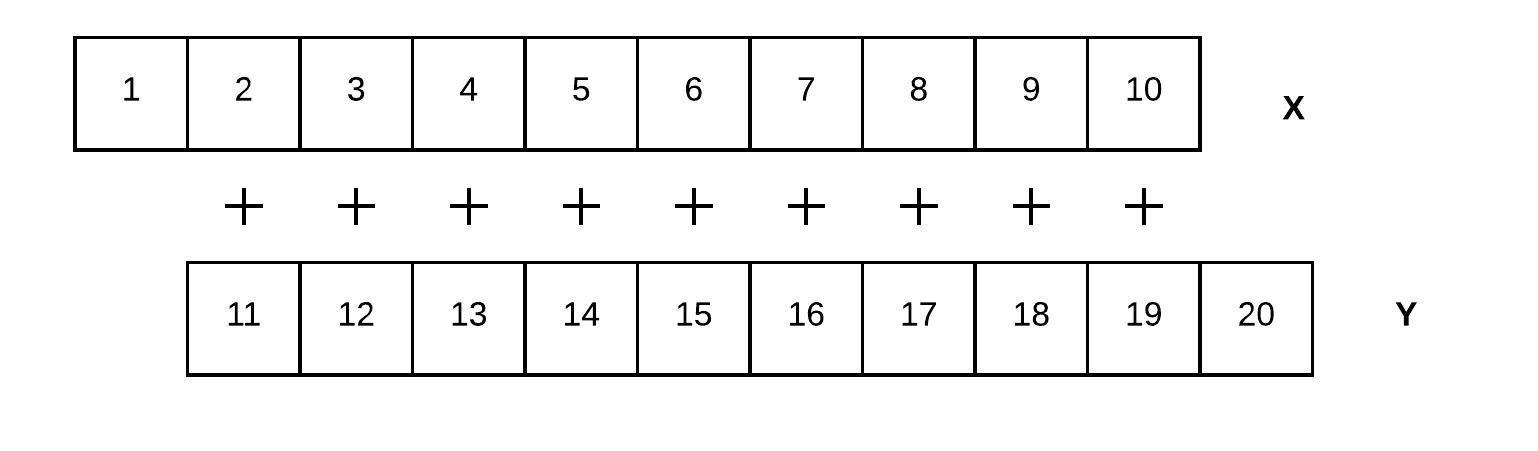
\includegraphics[width=7 cm]{./viz/ext/shiftAndAdd.jpeg}
 
 Note that you are allowed to use only one arithmetic operator
\end{DIY}

\begin{DIY}{Homework}
Given vector X and Y, compute $X^2$ without using the $\wedge$ operator
\end{DIY}

\subsubsection{Vectorizing with Comparison Operators}
\begin{knitrout}
\definecolor{shadecolor}{rgb}{0.969, 0.969, 0.969}\color{fgcolor}\begin{kframe}
\begin{alltt}
\hlstd{X}\hlkwb{<-}\hlkwd{seq}\hlstd{(}\hlnum{1}\hlstd{,}\hlnum{10}\hlstd{)} \hlcom{## generate a sequence of numbers from 1 to 10}
\hlstd{Y}\hlkwb{<-}\hlkwd{seq}\hlstd{(}\hlnum{11}\hlstd{,}\hlnum{20}\hlstd{)} \hlcom{## generate a sequence of numbers from 11 to 20}
\hlstd{X} \hlopt{>} \hlstd{Y}    \hlcom{##check if X is greater than Y}
\end{alltt}
\begin{verbatim}
##  [1] FALSE FALSE FALSE FALSE FALSE FALSE FALSE FALSE FALSE FALSE
\end{verbatim}
\begin{alltt}
\hlstd{Y[}\hlnum{5}\hlstd{]}\hlkwb{<-}\hlstd{X[}\hlnum{5}\hlstd{]} \hlcom{##set the 5th element of Y equal to the 5th element of X}
\hlstd{X} \hlopt{==} \hlstd{Y} \hlcom{##check for equality between X and Y}
\end{alltt}
\begin{verbatim}
##  [1] FALSE FALSE FALSE FALSE  TRUE FALSE FALSE FALSE FALSE FALSE
\end{verbatim}
\end{kframe}
\end{knitrout}

\begin{DIY}{Think}
What is the return type of applying comparison operators on vectors
\end{DIY}

\subsubsection{Are All Values True?}
\begin{knitrout}
\definecolor{shadecolor}{rgb}{0.969, 0.969, 0.969}\color{fgcolor}\begin{kframe}
\begin{alltt}
\hlstd{X}\hlkwb{<-}\hlkwd{seq}\hlstd{(}\hlnum{1}\hlstd{,}\hlnum{10}\hlstd{)} \hlcom{## generate a sequence of numbers from 1 to 10}
\hlstd{Y}\hlkwb{<-}\hlkwd{seq}\hlstd{(}\hlnum{11}\hlstd{,}\hlnum{20}\hlstd{)} \hlcom{## generate a sequence of numbers from 11 to 20}
\hlkwd{all}\hlstd{(Y} \hlopt{>} \hlstd{X)}
\end{alltt}
\begin{verbatim}
## [1] TRUE
\end{verbatim}
\begin{alltt}
\hlstd{Y[}\hlnum{5}\hlstd{]}\hlkwb{<-}\hlstd{X[}\hlnum{5}\hlstd{]} \hlcom{##set the 5th element of Y equal to the 5th element of X}
\hlkwd{all}\hlstd{(Y} \hlopt{==} \hlstd{X)}
\end{alltt}
\begin{verbatim}
## [1] FALSE
\end{verbatim}
\end{kframe}
\end{knitrout}

\subsubsection{Which Values Are True?}
\begin{knitrout}
\definecolor{shadecolor}{rgb}{0.969, 0.969, 0.969}\color{fgcolor}\begin{kframe}
\begin{alltt}
\hlstd{X}\hlkwb{<-}\hlkwd{seq}\hlstd{(}\hlnum{1}\hlstd{,}\hlnum{10}\hlstd{)} \hlcom{## generate a sequence of numbers from 1 to 10}
\hlstd{Y}\hlkwb{<-}\hlkwd{seq}\hlstd{(}\hlnum{11}\hlstd{,}\hlnum{20}\hlstd{)} \hlcom{## generate a sequence of numbers from 11 to 20}
\hlkwd{which}\hlstd{(Y} \hlopt{>} \hlstd{X)}
\end{alltt}
\begin{verbatim}
##  [1]  1  2  3  4  5  6  7  8  9 10
\end{verbatim}
\begin{alltt}
\hlstd{Y[}\hlnum{5}\hlstd{]}\hlkwb{<-}\hlstd{X[}\hlnum{5}\hlstd{]} \hlcom{##set the 5th element of Y equal to the 5th element of X}
\hlkwd{which}\hlstd{(Y} \hlopt{==} \hlstd{X)}
\end{alltt}
\begin{verbatim}
## [1] 5
\end{verbatim}
\begin{alltt}
\hlstd{X[X}\hlopt{==}\hlstd{Y]} \hlcom{##return the element of X that is equal to Y.}
\end{alltt}
\begin{verbatim}
## [1] 5
\end{verbatim}
\end{kframe}
\end{knitrout}

\begin{DIY}{Homework}
Using one arithmetic operation on Y, transform Y in a way such that $all(X==Y)$ returns TRUE
\end{DIY}

\begin{DIY}{Homework}
Using one arithmetic operation on Y, transform Y in a way such that $all(X<Y)$ returns TRUE
\end{DIY}

\begin{DIY}{Homework}
Transform only the values of Y that are even numbers, in such a way that they are all less than X. Then compare them with their corresponding values in X to verify if they are less. Try to do this in as few steps as possible.
\end{DIY}


% !Rnw root = Introduction.Rnw
\newpage
%===============================
%===============================
\section{Data Frames}
%===============================
%==================================  
\subsection{Data sets in R}
%==================================  
\noindent R comes packaged with a list of data sets which can be viewed with the following command: 
\begin{knitrout}
\definecolor{shadecolor}{rgb}{0.969, 0.969, 0.969}\color{fgcolor}\begin{kframe}
\begin{alltt}
\hlkwd{library}\hlstd{(}\hlkwc{help} \hlstd{=} \hlstr{"datasets"}\hlstd{)}
\end{alltt}
\end{kframe}
\end{knitrout}
\noindent These data sets are a great starting point for new comers to try out different R expressions on, and getting your hands dirty. 
%==================================  
\subsection{View a data set}
\subsubsection{The $View()$ function}
%==================================  
\noindent The $View()$ function can be used to see the contents of a data set wherein the argument to the function is the object that contains the data.
\begin{knitrout}
\definecolor{shadecolor}{rgb}{0.969, 0.969, 0.969}\color{fgcolor}\begin{kframe}
\begin{alltt}
\hlkwd{View}\hlstd{(iris)} \hlcom{##see the contents of a data frame}
\end{alltt}
\end{kframe}
\end{knitrout}
%==================================  
\subsection{Type of an Data Frame}
\subsubsection{The $class()$ function}
%==================================  
\noindent We can get the type of an R object by using the $class()$ function. This is synonymous to using the $DESC()$ function in your SQL query  
\begin{knitrout}
\definecolor{shadecolor}{rgb}{0.969, 0.969, 0.969}\color{fgcolor}\begin{kframe}
\begin{alltt}
\hlkwd{class}\hlstd{(iris)} \hlcom{## get the type of a data frame}
\end{alltt}
\begin{verbatim}
## [1] "data.frame"
\end{verbatim}
\end{kframe}
\end{knitrout}
%==================================  
\subsection{Size of a Data Frame}
\subsubsection{The $dim()$ function}
%==================================  
\noindent For objects that have a tabular structure, the $dim()$ function enables us to get the number of rows (observations) and number of columns (attributes)  
\begin{knitrout}
\definecolor{shadecolor}{rgb}{0.969, 0.969, 0.969}\color{fgcolor}\begin{kframe}
\begin{alltt}
\hlkwd{dim}\hlstd{(iris)} \hlcom{##get the dimensions (number of rows,number of columns)}
\end{alltt}
\begin{verbatim}
## [1] 150   5
\end{verbatim}
\end{kframe}
\end{knitrout}
\noindent Now,try:
\begin{knitrout}
\definecolor{shadecolor}{rgb}{0.969, 0.969, 0.969}\color{fgcolor}\begin{kframe}
\begin{alltt}
\hlkwd{class}\hlstd{(}\hlkwd{dim}\hlstd{(iris))} \hlcom{##get the class of the object returned by}
\end{alltt}
\begin{verbatim}
## [1] "integer"
\end{verbatim}
\begin{alltt}
\hlcom{##the call to dim() function}
\end{alltt}
\end{kframe}
\end{knitrout}
\begin{DIY}{Think}
Do you see the difference in result when iris is passed as an argument to $class()$ v/s when $dim(iris)$ is passed as an argument to $class()$. Think about what does the output signify?   
\end{DIY}

\begin{DIY}{Think}
Did you notice how $class()$ takes a data.frame as an argument in one case while takes $dim(iris)$ in another. Relate this observation to the ideas of objects and encapsulation that we have discussed until now.   
\end{DIY}

\begin{DIY}{Homework}
Get only the row count of the data set
\end{DIY}

%==================================  
\subsection{Attribute of a Data Frame}
\subsubsection{The \textbf{\$} operator}
%==================================  
\noindent Attributes of an R object can be accessed by the \textbf{\$} operator. This operator is synonymous to selecting a column in a spreadsheet or a database table.
\begin{knitrout}
\definecolor{shadecolor}{rgb}{0.969, 0.969, 0.969}\color{fgcolor}\begin{kframe}
\begin{alltt}
\hlstd{resut}\hlkwb{<-}\hlstd{iris}\hlopt{$}\hlstd{Sepal.Length} \hlcom{##acessing columns of a data frame}
\end{alltt}
\end{kframe}
\end{knitrout}
%==================================  
\subsection{Create a Histogram}
\subsubsection{The $hist()$ function}
%==================================  
\noindent A histogram which plots the number of occurrences of distinct elements (\textbf{\emph{discrete variables}}) in the attribute or number of occurrences of distinct intervals (\textbf{\emph{continuous variables}}) in the attribute.
\begin{knitrout}
\definecolor{shadecolor}{rgb}{0.969, 0.969, 0.969}\color{fgcolor}\begin{kframe}
\begin{alltt}
\hlkwd{hist}\hlstd{(iris}\hlopt{$}\hlstd{Sepal.Length)} \hlcom{##create a histogram of sepal sength which}
\end{alltt}
\end{kframe}
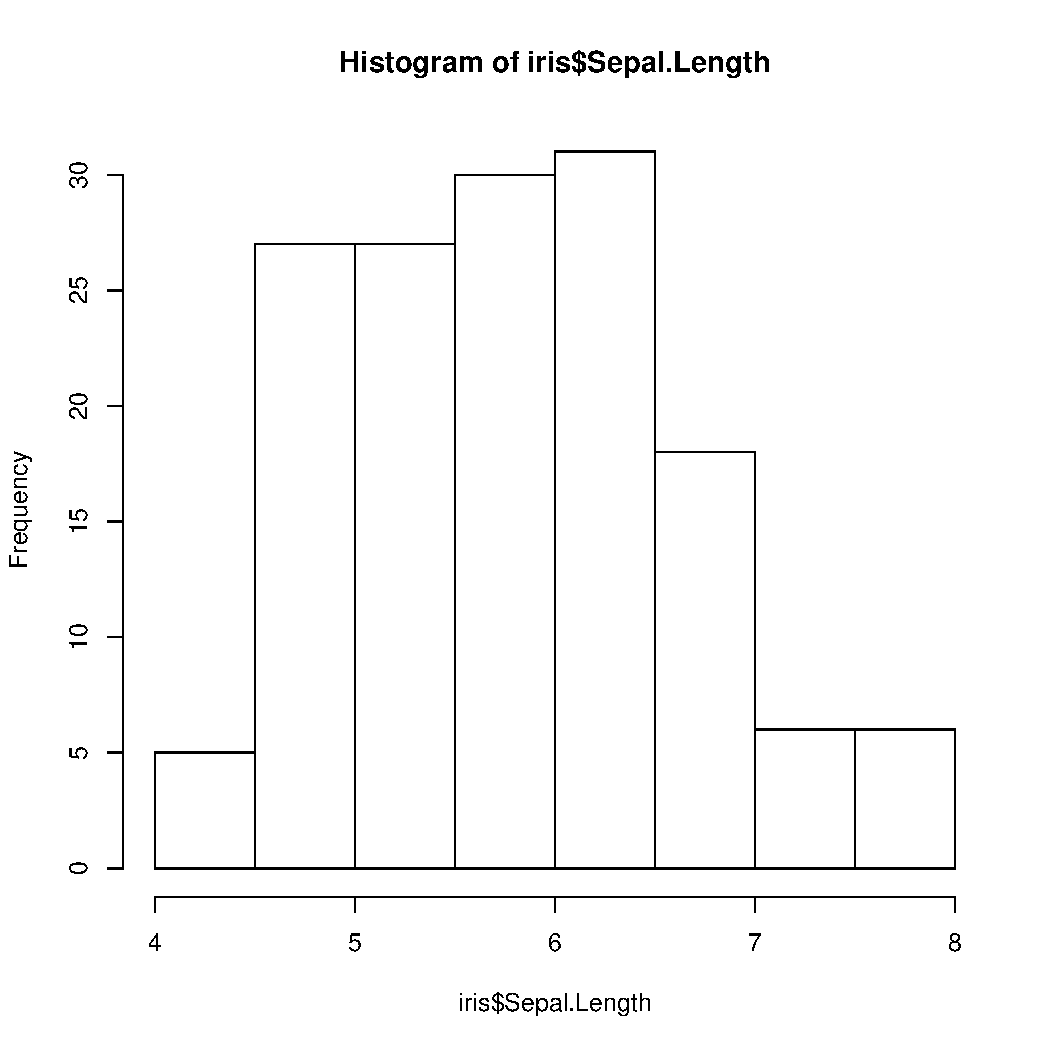
\includegraphics[width=\maxwidth]{figure/hist-1} 
\begin{kframe}\begin{alltt}
\hlcom{##is a vector of the numeric class}
\end{alltt}
\end{kframe}
\end{knitrout}

\begin{DIY}{Think}
Is the argument passed to $hist()$ a \emph{discrete attribute} or a \emph{continuous attribute}? Explain your choice.
\end{DIY}

\begin{DIY}{Think}
Change the histogram plot to show normalized frequencies
\end{DIY}

\begin{DIY}{Homework}
Find the sum of the first 10 and last 10 sepal lengths.
\end{DIY}
%==================================  
\subsection{Create a Scatterplot}
\subsubsection{The $plot()$ function}
%==================================  
\noindent The plot function takes two numeric arrays as arguments and treats each pair of values in the in the arguments as $(X,Y$ coordinates, thereby producing a scatter plot 
\begin{knitrout}
\definecolor{shadecolor}{rgb}{0.969, 0.969, 0.969}\color{fgcolor}\begin{kframe}
\begin{alltt}
\hlkwd{plot}\hlstd{(cars}\hlopt{$}\hlstd{speed,cars}\hlopt{$}\hlstd{dist)} \hlcom{##create a scatter plot with speed on the x axis}
\end{alltt}
\end{kframe}
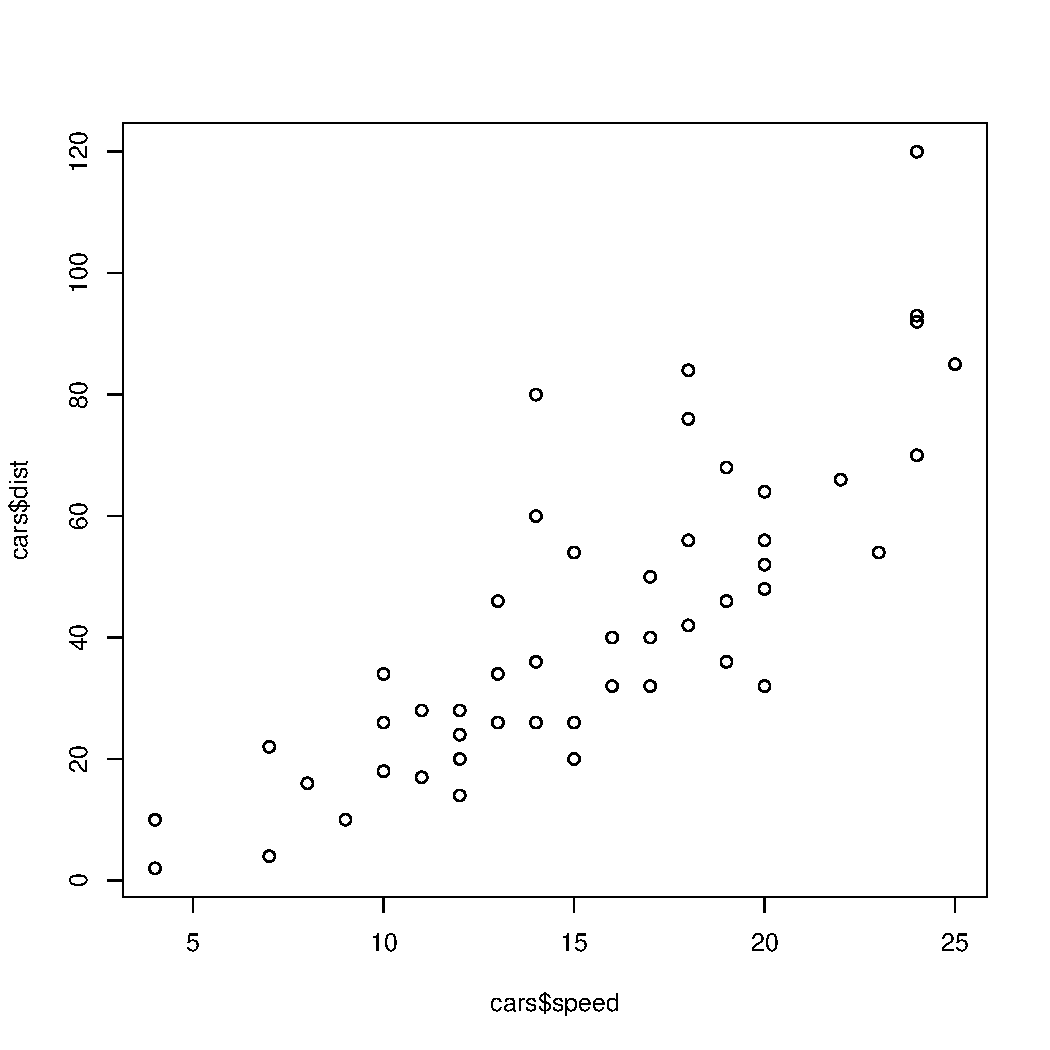
\includegraphics[width=\maxwidth]{figure/plot-1} 
\begin{kframe}\begin{alltt}
\hlcom{## and distance on the y axis}
\end{alltt}
\end{kframe}
\end{knitrout}

\begin{DIY}{Think}
Can you \emph{explain} the plot that you see above?
\end{DIY}

\begin{DIY}{Think}
Change the markers in the plot from circles to crosses. Moreover change the of the markers
\end{DIY}

\begin{DIY}{Think}
What will you get when you pass a data frame with three attributes as an argument to the $plot()$ function
\end{DIY}

%==================================  
\subsection{Create a Data Frame}
%==================================  
\begin{knitrout}
\definecolor{shadecolor}{rgb}{0.969, 0.969, 0.969}\color{fgcolor}\begin{kframe}
\begin{alltt}
\hlstd{X}\hlkwb{<-}\hlkwd{data.frame}\hlstd{(}\hlkwd{c}\hlstd{(}\hlnum{1}\hlstd{,}\hlnum{2}\hlstd{),}\hlkwd{c}\hlstd{(}\hlstr{"apples"}\hlstd{,}\hlstr{"oranges"}\hlstd{),}
              \hlkwd{c}\hlstd{(}\hlnum{TRUE}\hlstd{,}\hlnum{FALSE}\hlstd{))}  \hlcom{##adding data to a data frame wherein }
\hlcom{##each vector represents a column of the deta frame}
\hlstd{X}
\end{alltt}
\begin{verbatim}
##   c.1..2. c..apples....oranges.. c.TRUE..FALSE.
## 1       1                 apples           TRUE
## 2       2                oranges          FALSE
\end{verbatim}
\begin{alltt}
\hlkwd{names}\hlstd{(X)}\hlkwb{<-}\hlkwd{c}\hlstd{(}\hlstr{"id"}\hlstd{,}\hlstr{"fruits"}\hlstd{,}\hlstr{"has_vitaminC"}\hlstd{)} \hlcom{##adding attribute names }
\hlcom{##to the data frame}
\hlstd{X}
\end{alltt}
\begin{verbatim}
##   id  fruits has_vitaminC
## 1  1  apples         TRUE
## 2  2 oranges        FALSE
\end{verbatim}
\begin{alltt}
\hlstd{X}\hlopt{$}\hlstd{fruits}
\end{alltt}
\begin{verbatim}
## [1] apples  oranges
## Levels: apples oranges
\end{verbatim}
\end{kframe}
\end{knitrout}

\begin{DIY}{Think}
The output for the last expression shows that the attribute fruits has levels. What does this mean?
\end{DIY}

\begin{DIY}{Homework}
Pick a data set from the list of available data sets and \emph{explore it} using the \emph{R expressions} you have just learnt.
\end{DIY}

\begin{DIY}{Homework}
Create a data frame for the example shown in section \ref{sec:GeomOfData} and generate the plot that was shown in the same section.
\end{DIY}


% !Rnw root = UsingR.Rnw
\newpage
%===============================
\section{Input/Output with External Sources}
%===============================
\begin{HIGHLIGHT}
\par\noindent{
Reading in data from files like ``\textbf{.txt}'',``\textbf{.csv}'' and ``\textbf{.xls}'' into the R environment has been greatly simplified by RStudio. Just goto  Environment tab $->$ Import Dataset  and select the file type from which you want to import the data (for \emph{.txt} and  \emph{.csv} files choose the ``From CSV...'' option while for excel sheets choose ``From Excel..'' option). A new window will open up with a set of options that will guide you to import your data in R.        
}
R also provides a set of functions for reading and writing data. An inquisitive reader can read about them in \textcolor{cyan}{\url{https://www.datacamp.com/community/tutorials/r-tutorial-read-excel-into-r}}
\end{HIGHLIGHT}

\begin{DIY}{Think}
Though RStudio has simplified the process of reading in data by providing a GUI, it hasn't provided any mechanism for writing data out of the R environment. What do you think this is the reason for this?  
\end{DIY}

\begin{DIY}{Homework}
Do the following
\begin{enumerate}
  \item Remove the headers from exercise1.csv and try importing it into the R environment. What do you observe?
  \item Replace exercise1.csv as exercise1.tsv (i.e change the delimiter between attributes from comma to tab) and try importing it into the R environment.
\end{enumerate}
\end{DIY}
%===============================
\subsection{IO with RDBMS}
%===============================
%=============================
\begin{figure}[ht]
 \centering
    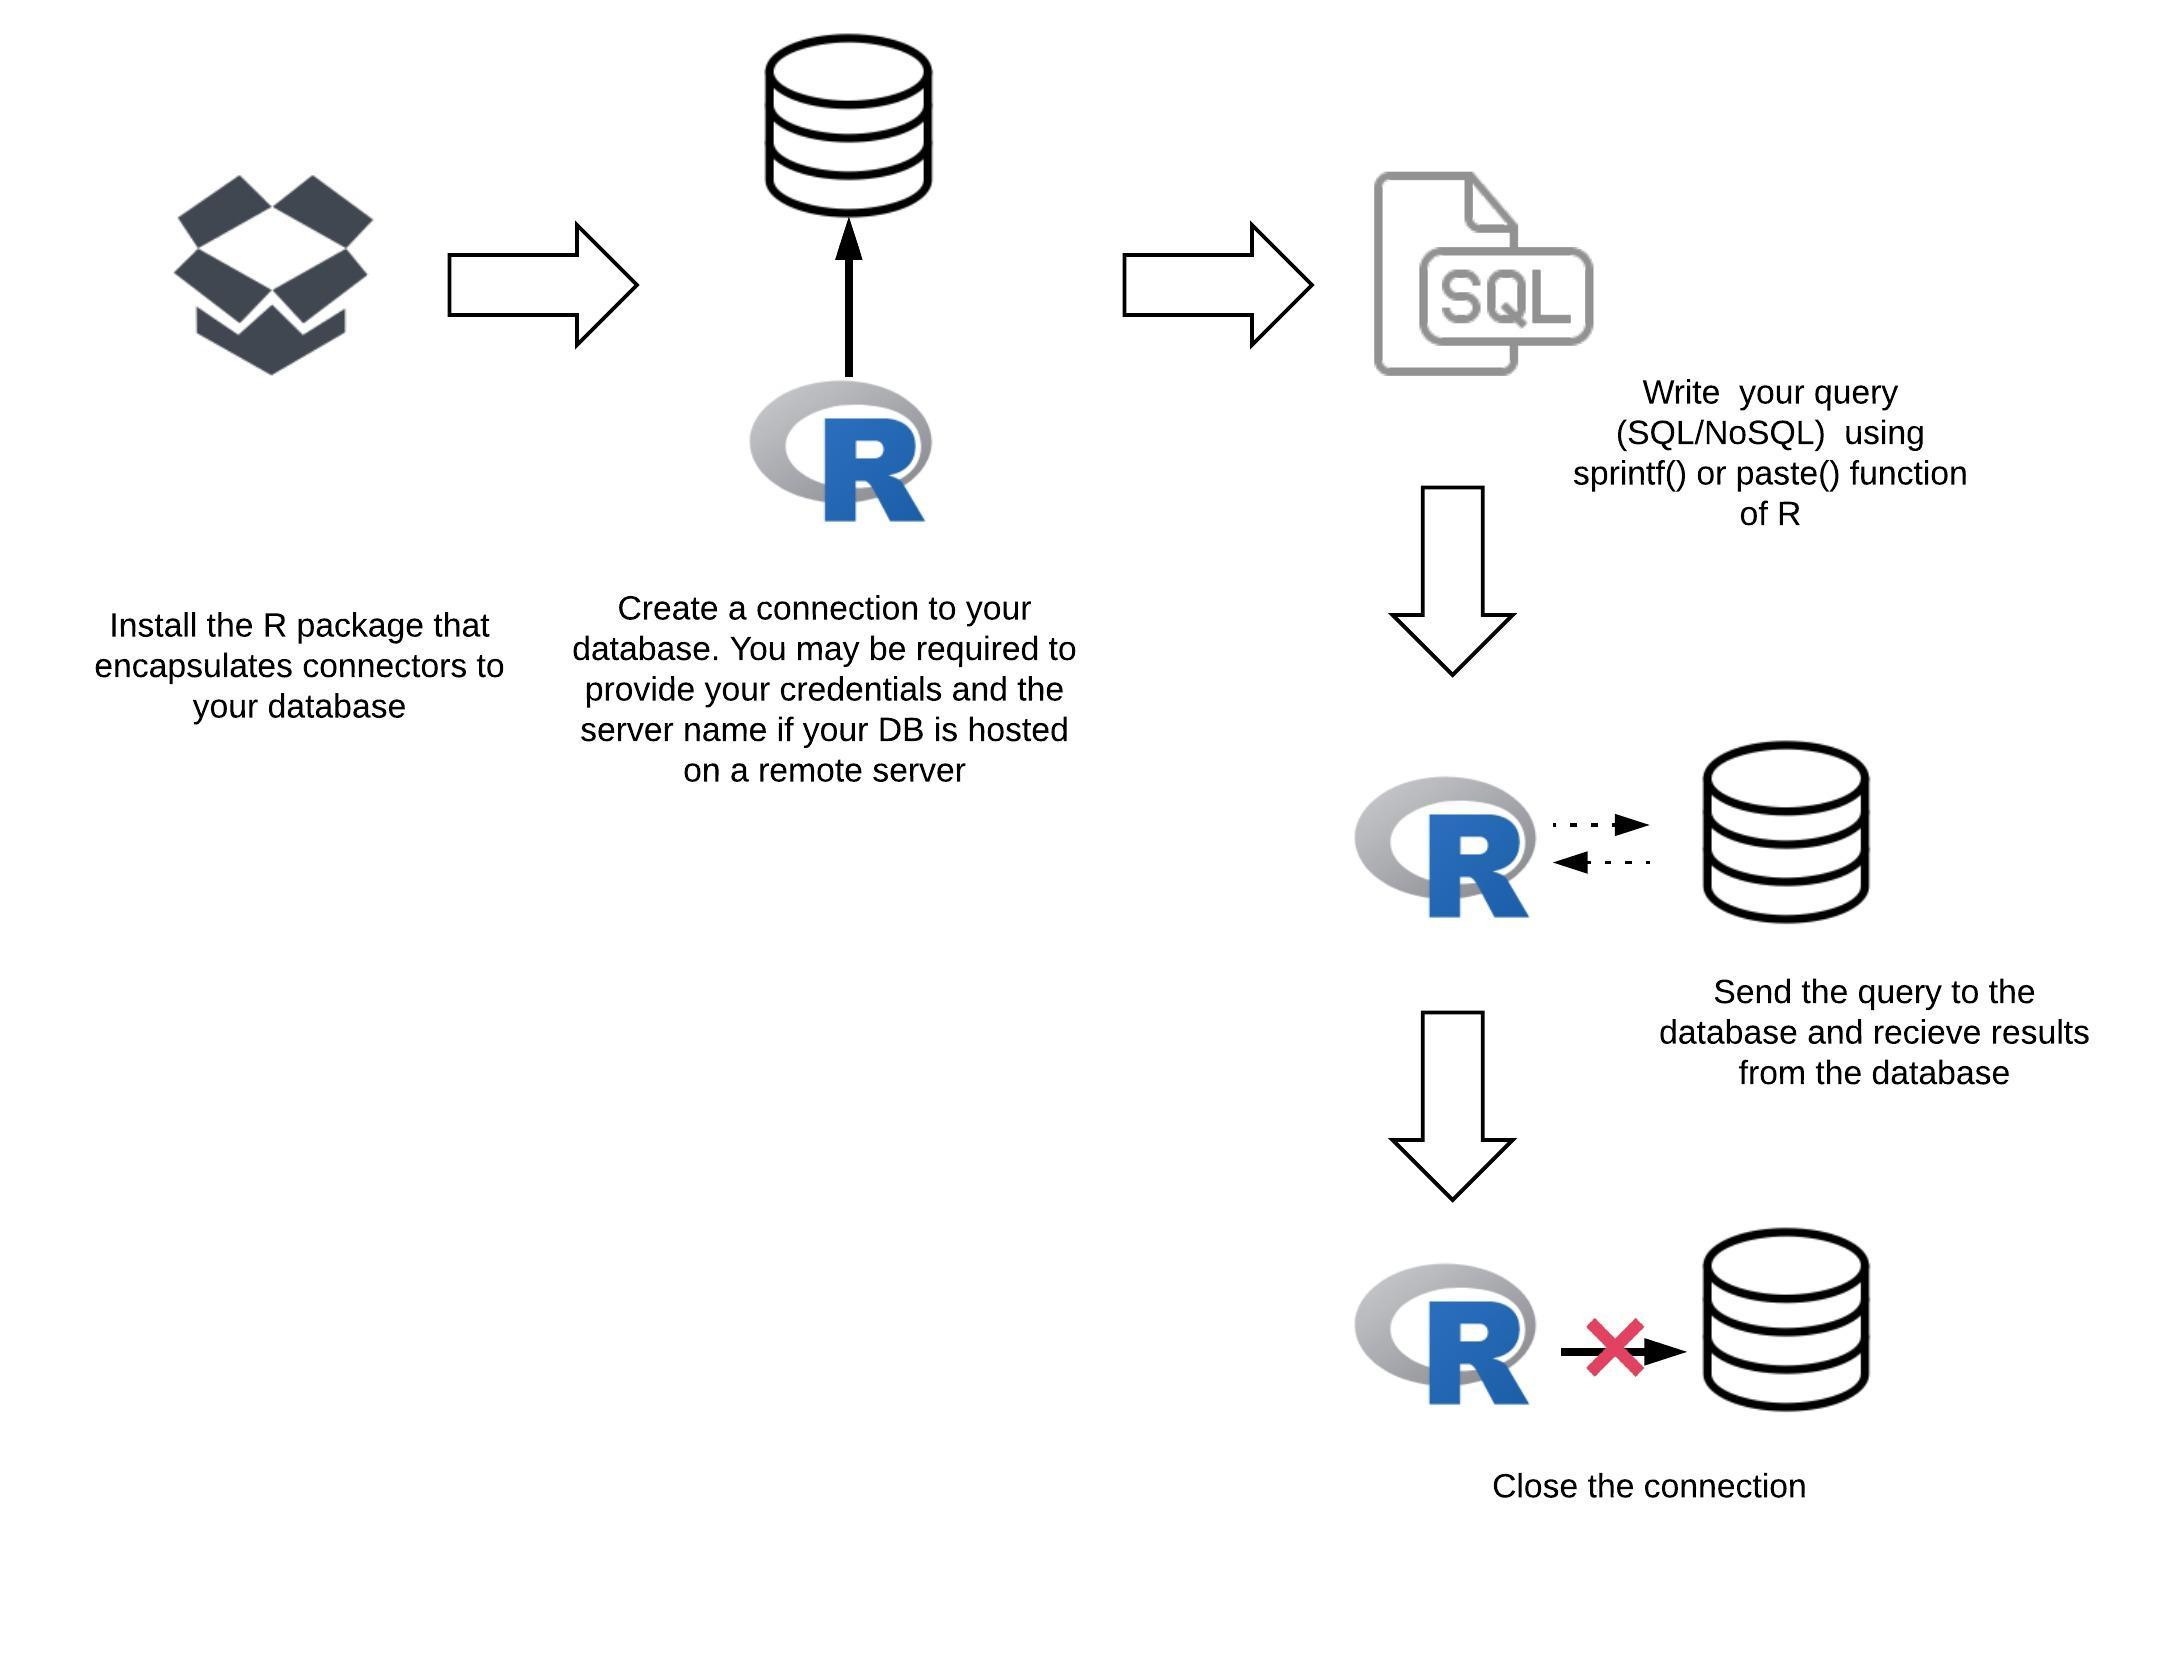
\includegraphics[width = 15 cm]{./viz/ext/IO_R_RDBMS.jpeg}
\end{figure}
\begin{HIGHLIGHT}
A large number of different databases exist in the market and each of them has is its own way of setting up and managing connections with client applications. These low level connection details are encapsulated by R packages and the user only has to be aware of an abstract view as shown in the schematic. Details of R packages for connecting to some of the popular databases can be found in the following links:
\begin{itemize}
  \item How to Connect to an Oracle Database:
  
  \textcolor{cyan}{\url {http://rprogramming.net/connect-to-database-in-r/}}
  \item How to Connect to a MySQL Database:
  
  \textcolor{cyan}{\url {https://www.r-bloggers.com/mysql-and-r/}}
  \item How to Connect to MongoDB: 
  
  \textcolor{cyan}{\url {https://www.r-bloggers.com/r-and-mongodb/}}
\end{itemize}
\end{HIGHLIGHT}

As, shown in the schematic, SQL queries can be constructed with the $sprintf()$ and $paste()$ function. We give a few examples here:
\begin{knitrout}
\definecolor{shadecolor}{rgb}{0.969, 0.969, 0.969}\color{fgcolor}\begin{kframe}
\begin{alltt}
\hlkwd{sprintf}\hlstd{(}\hlstr{"select * from names where name in (%s)"}\hlstd{,}
        \hlkwd{paste}\hlstd{(}\hlkwd{c}\hlstd{(}\hlstr{"'Andrew"}\hlstd{,}\hlstr{"John"}\hlstd{,}\hlstr{"Jane'"}\hlstd{),}\hlkwc{collapse}\hlstd{=}\hlstr{"','"}\hlstd{)}
       \hlstd{)}
\end{alltt}
\begin{verbatim}
## [1] "select * from names where name in ('Andrew','John','Jane')"
\end{verbatim}
\begin{alltt}
\hlkwd{sprintf}\hlstd{(}\hlstr{"insert into networks (id, name) values (%d, '%s');"}\hlstd{,}
                    \hlnum{11}\hlstd{,} \hlstr{"John"}
        \hlstd{)}
\end{alltt}
\begin{verbatim}
## [1] "insert into networks (id, name) values (11, 'John');"
\end{verbatim}
\end{kframe}
\end{knitrout}

\begin{DIY}{Warning}
Yes, it is indeed complicated to write queries in R as compared to writing them in a SQL editor. But the idea is to realize, as a user that one should do complicated aggregations and transformation of the data either solely in the database and store it back in tables where R can query from or within R itself (after having imported the data) but \textbf{NEVER} at the interface level. \emph{Complicated interfaces lead to unmanageable software}.When you have large amounts of data, trying to read in all the data of the database into R and then doing the data aggregation and transformation in R is also \textbf{NOT} a good idea as it creates a lot of dependency on the connector between R and the database which may have its own limitations based on how it has been implemented.  
\end{DIY}
